\cleardoublepage
\chapter{System Architecture} \label{chap:sysArch}
\todo[inline,color=red!40]{*Chapter Introduction}
\todo[inline,color=blue!40]{*1-System Elements}
\todo[inline,color=blue!40]{     *1-The sensors/Actuator}
\todo[inline,color=blue!40]{     *2-The processing Unit}
\todo[inline,color=blue!40]{     *3-Processing type?}
\todo[inline,color=blue!40]{*2-Architecture proposal}
\todo[inline,color=blue!40]{*3-Approach to the problem}
\section{System Elements}
In order to develop a system that is able to properly measure and return an good approximation of the liquid level in the LPG bottle, is necessary to identify the elements that must be present in the system. With this information, we must be able to properly chose the components to the system, to develop a solution that fits in the purpose of the work. In Chapter \ref{chap:stArt}, several methods/techniques were presented to measure the liquid level inside a LPG bottle, from those the choice fell to the development of a system that analyses the transversal vibration in the LPG bottle, with this in consideration is easier to define the elements that should be part of the system. 
\subsection*{Actuator}
This element is  responsible for the stimulation of the system, is very important that the chosen actuator is capable to produce the transversal vibration in the system. For this specific case, were presented two different methods for that purpose.
\subsection*{Sensor}
The amount of sensors that can be used to measure the vibration, not specific to this case only, is very wide. There were presented several types of sensors already, but when choosing a specific one it must be taken into consideration aspects like is practical application, in this case, the dimensions of the sensor, his cost and the coupling with the system to be measure, as an example. Other aspects that should be taken in consideration when choosing the sensor, are specific to the sensor itself and may vary from one to another, is not relevant to specify them. 
\subsection*{The Processing Unit}
The selection of the processing unit is quite important, since is the "brain" of the entire system. First of, is responsible for capturing the signal from the sensors, process the signals and at the end being able to return to the user some information, relevant for the application, for this particular application must return some data that is proportional to the liquid level. The processing unit in this case must be equipped with different types of I/O ports, for the specific case, the most important are the ADC for converting the continuous time signal to a discrete signal. Beside the I/O, the system must have the computational power to perform any type of mathematical tasks needed in the signal processing, isn't necessary to have a dedicated DSP hardware, but should be able to perform those tasks in a reasonable period of time.  
%Not sure if it should be here
\todo[inline,color=red!40]{Should be here?}
\subsection*{Processing Type}
As a signal is converted and stored in the processing unity, the signal is decomposed in two variables, they are the dependent variable and the independent variable, the first is usually related with the amplitude of the signal and the other with the sample and overall can be seen as the output of a sensor at a certain moment of time. While this data can be used to return a visual information about the state of the sensor, is not the only way, is often used the frequency domain, to determine patterns in the response of the same sensor, that aren't clear in a time domain visualization.

\section{Architecture proposal}
The system architecture consist in the union of the elements mentioned, to obtain device capable of measure what is intended to. The device itself should be attached in each LPG bottle, to be able to return to the user the liquid level inside. The figure \ref{fig:systemArch} is a illustration of the system elements on the device.\\
\begin{figure}[!htb]
    \centering
    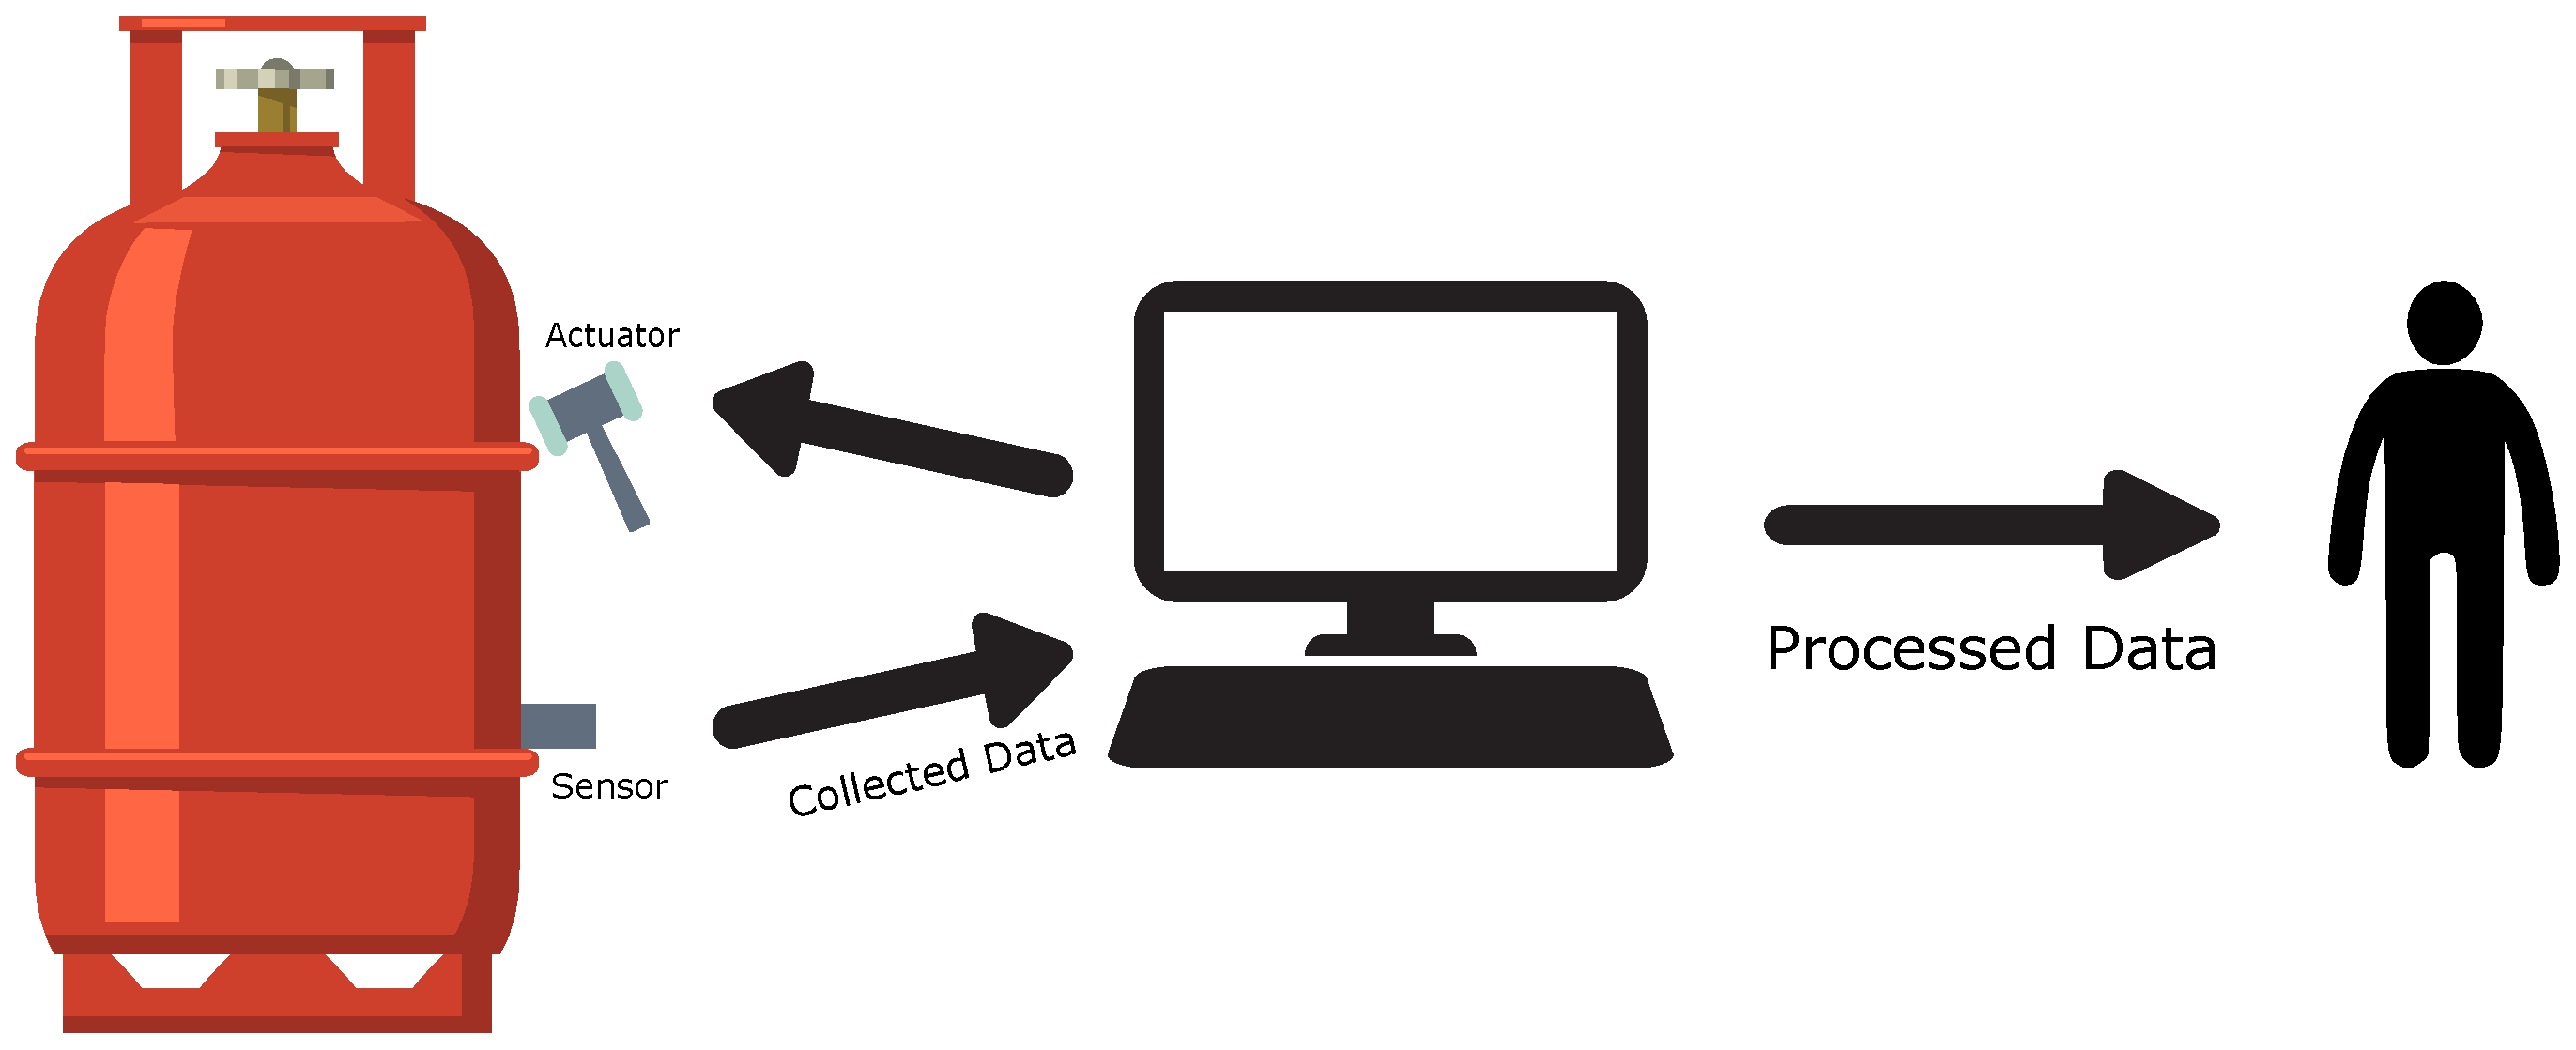
\includegraphics[width=0.55\textwidth]{Chapters/3CHP/Images/bottleBaseAct.eps}
    \caption{Basic architecture of the liquid level measuring device}
    \label{fig:systemArch}
\end{figure}
In the device, the processing unit is responsible for the control of the system as well, the unit is responsible for trigger the actuator in the first place, when this happens the hammer hits the side surface of the LPG bottle and thus the vibration is produce. In the mean time, the process unit starts to convert the signal from the sensor and store that value. Then the recorded data must be processed, in order to return to the user the desire information. Ideally, this procedure would occur once or twice a day, unless a manual measure was requested by the user, but for the purpose of the development of the device, the main purpose is to, in a first stage to get information and being able to associate the same information to the liquid level.\\
The chosen method to process the information, is throw the analysis of the acquired data in the frequency domain, for that a FFT is the chosen method to process the data and later be able to observe and associate the same information with the liquid level. A brief and visual description of the flow of how the process is suppose to occur in the processing unit is illustrated in  
\begin{figure}[!htb]
    \centering
    %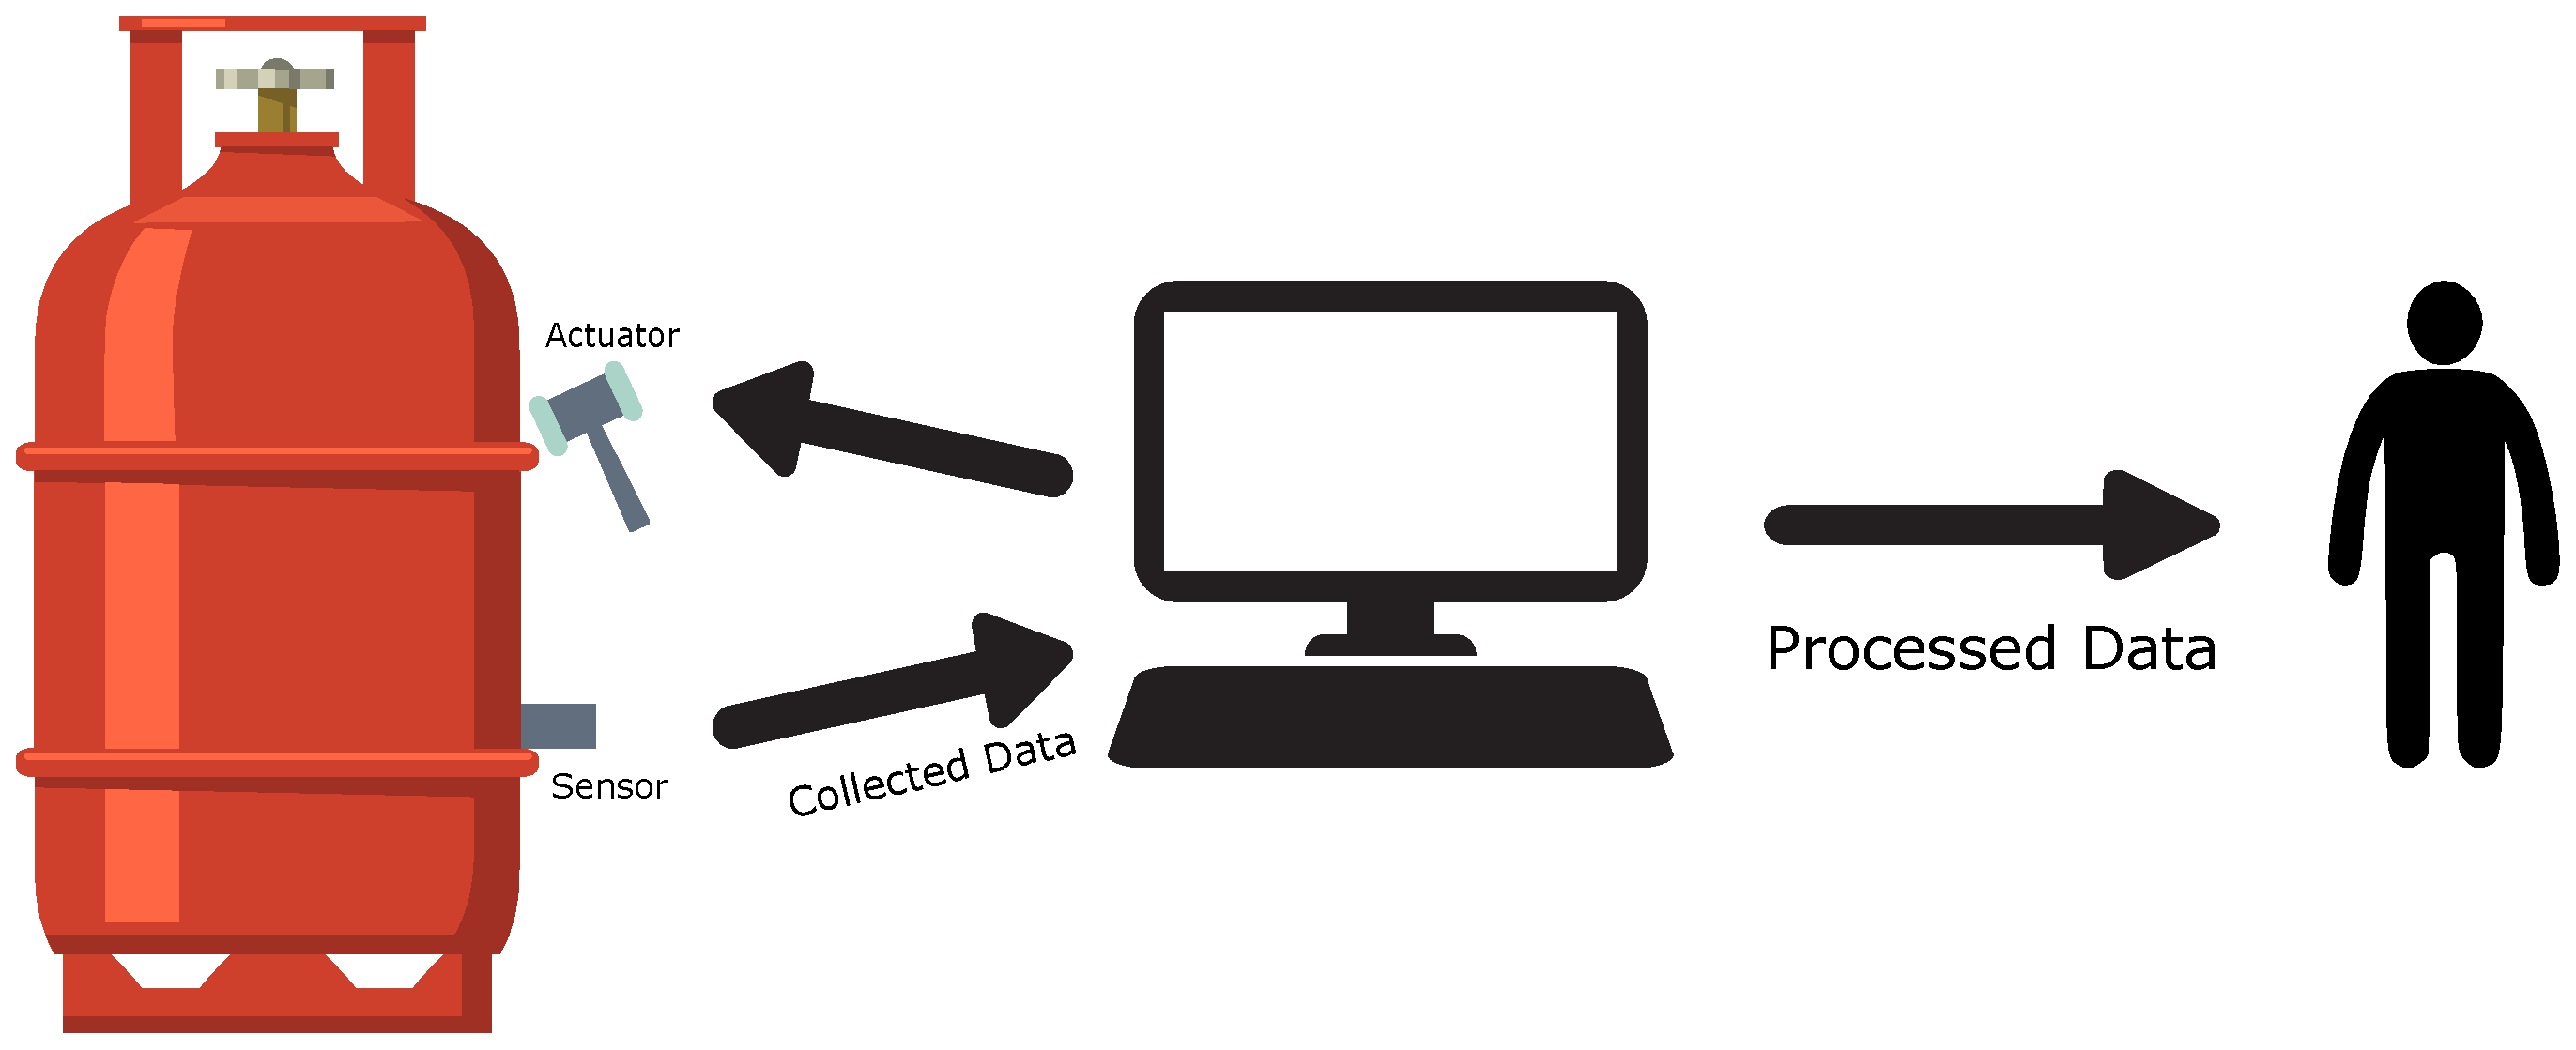
\includegraphics[width=0.65\textwidth]{Chapters/3CHP/Images/bottleBaseAct.eps}
    \caption{Proposed diagram for the device operation}
    \label{fig:systemSWFlow}
\end{figure}\\
\todo[inline,color=red!40]{Should I explain the diagram, or isn't necessary from the explanation before the ilustration?}

\section{Problem Approach}
The approach to obtain a solution and hopefully a device capable of measuring correctly the LPG liquid level will be split in two main phases, each one of them with a different purpose, they are the study of behavior of the system to a external stimulation and the development of the solution for this case. In the two phases the Hardware selection will be different, but on the other hand to what concerns the data processing will be a mixture of different approaches.
In the first stage and in order to understand the behavior, limit the range of analysis of the data and define to the LPG bottle a maximum and minimum value of liquid, it will be used a hammer, a microphone and a computer installed with MatLab, this will allow to capture the sound produced when hitting the side surface of the LPG bottle, and process it in MatLab with the FFT function to analyze the spectrum of the acquired data.
The second stage will be divided in several smaller steps, so is possible to mislead any source of problems. In this stage the microphone will be replaced with two sensors, with the same purpose, in a first stage the hammer will continue to be used as a stimulation method, although later will be replaced with a solenoid, in order to perform automatically the trigger and the signal acquisition. In the same way, in the beginning MatLab will still be used to process the data, but later is to use a microcontroller for that purpose, although for capturing the signals from the sensors, a microcontroller will be used as the interface, and then send the data to the computer. The reason for this is that this way is easier to understand the type of signals acquired from the sensors and how is the proper way to process this data later, on a implementation, avoiding skipping steps.
\todo[inline,color=red!40]{Should  I add a time-table for the approach?}

%everything bellow this will later be migrated to a different chapter - Don't forget to change
\section{Introduction}
%check if the last section of the previous chapter is the more appropriate to use here
%a brief sum of what is going to be presented in this chapter, i.e., first the presentation of the sensors, then the micro controller in use, them the circuits, and at the end the mounting for each case. For what is related to the accelerometer and piezo, both the setups, the simplest and with the pieces.
\section{Hardware selection}%%change this section name later
The analysis through vibration, is the chosen approach to measure the amount of liquid gas inside the LPG bottle, since the stimulation of the system is by hitting in the surface of the bottle, beside the vibration this will produce a characteristic sound as well. From this, 3 different sensors where chosen to acquire the signals when hitting the surface of the LPG bottle, they are a microphone, a piezoelectric sensor and a MEMS accelerometer.\\
In all the cases, when hitting the surface of the bottle with a hammer, this will produce a characteristic vibration and sound, in order to characterize the response of the system to the hit of the hammer, the first analysis is made with a microphone, after this the sensors will be chosen and the design the appropriate circuit to capture the same signal.
%%Incomplete, must be able to include references to the microcontroller and the circuits

\subsection{Microphone}
Before trace a curve is important to understand which one is the best point to acquire data, when hitting the surface of the bottle. For that, different point in the bottle were chosen to determine the point. After this several measurements must be conducted in order to have a reliable source of information and trace a curve for the system response.\\
The point considered are in the side surface of the LPG bottle as illustrated in the following image:
%%insert here a description of the points considered
To make those measurements a setup must mounted with a microphone, to capture the sound produced and process it. The setup is quite simple, consisting in a microphone and a computer installed with MatLab. The microphone in use is from a phone and to connect it with the computer an software called \textit{WO Mic}, this allows to used the microphone of the phone in real-time. The software must be installed in both devices, in the phone the software is available for Android and IOS, is responsible to transmit what is captured from the microphone. In the computer the client application and a virtual device must be installed to use the Phone in the computer to perform any type of tasks, this connection can be made by USB, Bluetooth, Wi-Fi and Wi-Fi Direct.\\ 
In order to save what is captured from the microphone, the software is split in three main block with different purposes, the \textit{WO Mic App} runs in the Phone, samples the input of the microphone and transmit it to the computer, the \textit{WO Mic Client}, runs in the computer, connect to the app in the phone, and receive the data from the microphone, which is transmitted to the \textit{WO Mic Virtual Device} on which a real microphone device is simulated and provides the audio to any application or program in the computer\cite{WOMicFREE}:\\
\begin{figure}[!htb]
    \centering
    \includegraphics[width=0.65\textwidth]{Chapters/3CHP/Images/WOMICDiag.png}
    \caption{Flow of data in the components of the software\cite{WOMicFREE}}
    \label{fig:diagramWOMIC}
\end{figure}
In addition to this, is also necessary to install the drivers of the phone in use, if the connection is made over USB.\\
To save the acquired data, MatLab was used to record the data of the microphone from the desire time and saved in ".txt" files for further analysis. 
%%The following two paragraphs must go in other section
%%Insert flux gram here for a easy explanation and perception of the flow of information
A script in MatLab was developed in order to perform this measurements and the capture is made once at a time, but not all configurations are done over this script. To start, the phone is connected over USB to the computer, in the application at phone the transport selected must be \textbf{USB}, on the app settings and after that started the application, in the top right play shape button. 
%%Insert here instructions
In the computer the client software must be initialized and connected to the phone in the following order \textit{\>Connection\>Connect...} a new window will open, on which the \textbf{USB} must be selected as transport type and finalizing by pressing \textit{Connect}. In MATLAB the input correspondent to the microphone must be selected.\\
When this is done, the script runs and starts to record data from the microphone, for the desire amount of time. When the microphone starts to record, the surface of the LPG bottle is knocked and the captured signal is saved.
%%
%%
\subsection{Accelerometer}
As already mentioned in \ref{sec:VibSens}, there are various types of accelerometers, however the choice of the one to use depends on various factors, for this particular application is important that the accelerometer in use has a low cost and a small size, for the future application. With this in mind the choice declines over MEMS accelerometers, that are smaller when compared with piezoelectric accelerometers.\\
The type of MEMS accelerometers available is very wide, some of them started to be used in applications that usually uses piezoelectric accelerometers, like condition-based monitoring (CBM), structural health monitoring (SHM), asset health monitoring (AHM), vital sign monitoring (VSM) and IoT, for example. When selecting the accelerometer is important to take into consideration some parameters, which are responsible to determine the category of the accelerometer, they are the application, the bandwidth and the range. Although there is no standard for the category on each accelerometer fits in, \textit{Analog Devices} has one document where they divide their products in different categories, with the type of application used in each on of them featuring a description of the key parameters that must be taken into consideration when selecting the appropriate accelerometer.
\begin{figure}[!htb]
    \centering
    \includegraphics[width=1\textwidth]{Chapters/3CHP/Images/adTable.pdf}
    \caption{Application landscape for a selection of Analog Devices MEMS accelerometers}
    \label{fig:adtable}
\end{figure}
The MEMS accelerometers from \textit{Analog Devices} are divided in two families, the ADXLxxxx and the ADIS16xxxx, the last offers different advantages when compared with he first, more like a plug-and-play solution with features like factory compensation, embedded compensation and signal processing. This family obviously has one of the features that has particular interest for the application, in this case the fact that has signal processing on the accelerometer, on the other hand this comes with a price, and this family of products has a higher cost. So is necessary to define the key specifications of the accelerometer, in order to properly chose one\cite{AnalogDialogue51102017}\cite{AnalogDialogue51112017}.\\
The final purpose is to have a cheap and portable prototype, that is capable of accurately measure the vibrations and determine the the liquid level, this implies that his bandwidth covers the spectrum of frequency on which the curve of the relation liquid level vs frequency is. With this the key specifications are the low cost, low power and his bandwidth must close to 2kHz, determine as maximum frequency for a mechanical vibrations in \ref{tab:sampRat} and latter proved in the results obtained by \citeauthor{wuLiquidLevelDetector2014b} as described in \ref{sec:LPGModel}. Considering these specification, some models where chosen, that integrate this criteria, as follows:
\begin{table}
    \centering
    \includegraphics[width=1\textwidth]{Chapters/3CHP/Images/accTable.pdf}
    \caption{Key specifications of MEMS accelerometers}
    \label{fig:acctable}
\end{table}
Although is doesn't accommodate entirely the specifications but since it was already available for use, the choice fell to the ADXL335. This model offers a low power consumption of around 350$\mu$A, his bandwidth is adjustable with a single capacitor per axis, from 0.5 to 1600 Hz for X and Y axis and 0.5 to 550Hz for Z axis. Beside this the accelerometer itself is very cheap, with a price starting at 3€. To properly acquire the data from this sensor and process it, is necessary to integrate it with a amplifier circuit and a microcontroller, on which more details will be explain further ahead.
\subsection{Piezoelectric}
To what concerns in the choice of a piezoelectric sensor, although there are very types of this kind of transducers and there are various applications for them.  
\subsection{Amplifier circuits}
\subsection{Coupling} 

% \begin{figure}[!htb]
%     \centering 
%         \begin{subfigure}[c]{\textwidth}
%             \centering
%             \input{Sections/3Transforms/Images/DFTSymmetry.tex}
%             \caption{}
%             \label{subfig:dft}
%         \end{subfigure}
%         \begin{subfigure}[c]{0.45\textwidth}
%             \centering
%             \input{Sections/3Transforms/Images/DCT1Symmetry.tex}
%             \caption{}
%             \label{subfig:dct1}
%         \end{subfigure}
%         \begin{subfigure}[c]{0.45\textwidth}
%             \centering
%             \input{Sections/3Transforms/Images/DCT2Symmetry.tex}
%             \caption{}
%             \label{subfig:dct2}
%         \end{subfigure}
%         \begin{subfigure}[c]{0.45\textwidth}
%             \centering
%             \input{Sections/3Transforms/Images/DCT3Symmetry.tex}
%             \caption{}
%             \label{subfig:dct3}
%         \end{subfigure}
%         \begin{subfigure}[c]{0.45\textwidth}
%             \centering
%             \input{Sections/3Transforms/Images/DCT4Symmetry.tex}
%             \caption{}
%             \label{subfig:dct4}
%         \end{subfigure}
%         \caption{Sequences generated in the first step of Table \ref{tab:DFTDCT}for the DFT and different DCTs. Filled dots correspond to the original sequence ((a) - \emph{DFT}; (b)) - \emph{DCT-I}; (c)) - \emph{DCT-II}; (d)) - \emph{DCT-III}; (e)) - \emph{DCT-IV}).}
%     \label{fig:2NSeq}
% \end{figure}
% \begin{lstlisting}
%     ./aomenc <INPUT-FILE> -h <HEIGHT> -w <WIDTH> -o <OUTPUT-FILE> --limit=10 -p 1 --cpu-used=8 --i420 --q-hist=64 --end-usage=q --cq-level=<CQ-LEVEL>
% \end{lstlisting}
\clearpage
%\printbibliography[heading=subbibliography]
%\addcontentsline{toc}{section}{References}